\section{Introduction}
Generalised Parton Distributions (GPDs)
\cite{Mue94,Ji97a,Rad97} encompass the familiar parton
distribution functions (PDFs) and nucleon form factors to provide a
comprehensive description of the structure of the nucleon.
Although GPDs are difficult to access experimentally, the H{\sc ermes}
collaboration has previously published results
\cite{Air01,Air06,Air08,Air09,Air10, Air10a, Air10b, Air11} on
the leptoproduction of real photons from a nucleon or nucleus that can
be used to constrain GPDs via Compton Form Factors (CFFs).\red{ A thorough
desccription of the nucleon in terms of GPDs would allow the deduction
of the total angular momentum of partons in the nucleon and the
construction of a 
longitudinal-momentum dissected transverse spatial map of parton positions.}

Generalised parton distributions depend upon four kinematic variables: the
Mandelstam variable $t=(p-p^{\prime})^2$, which is the squared momentum
transfer to the target nucleon in the scattering process with $p$ ($p^{\prime}$)
representing the initial (final) four-momentum of the proton; the average
fraction $x$ of the nucleon's longitudinal momentum carried by the active
quark throughout the scattering process; half the difference \red{of
  the} fraction\red{s} of the nucleon's longitudinal momentum carried
by the active quark at the start and end of the process, written as
the skewness $\xi$; and the square $-Q^2=q^2$ of the four-momentum of
the virtual photon that mediates the lepton-proton scattering
process. In the Bjorken limit of $Q^2\rightarrow\infty$ with fixed
$t$, \red{the skewness} $\xi$ is related to the Bjorken variable
$x_{\textrm{B}}=\frac{-q^2}{2p\cdot q}$ as
$\xi\approx\frac{x_\textrm{B}}{2-x_\textrm{B}}$. The results are presented
\red{as a function of} $x_{\textrm{B}}$ because there is no consensus on an experimentally
observable representation of $\xi$. 

\begin{figure}
\begin{center}
\subfigure[DVCS]{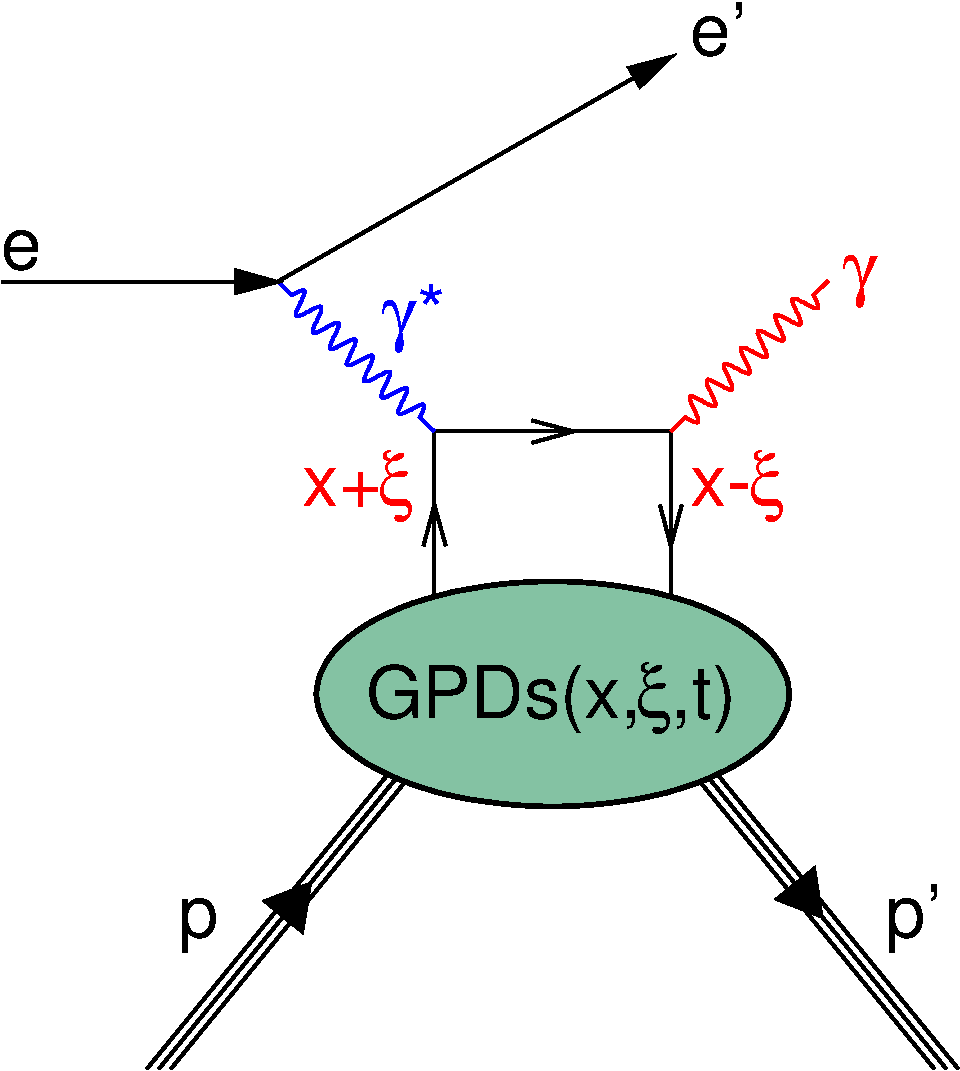
\includegraphics[width=5.6cm]{dvcs}}
\hspace{3cm}
\subfigure[Bethe Heitler]{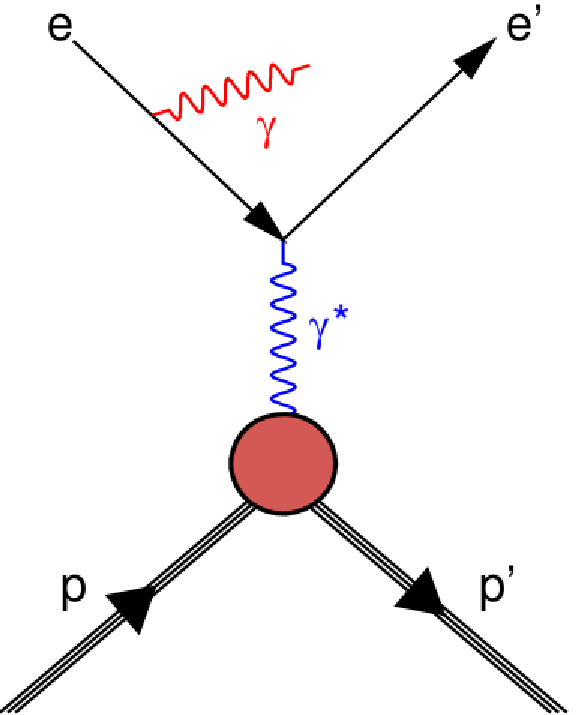
\includegraphics[width=5.2cm]{1_bh}}
\caption[DVCS and Bethe Heitler hand bag diagram.]{(a): The DVCS process in
which an electron/positron ($e$) interacts with a quark in the nucleon
($p$) via a virtual photon ($\gamma^\ast$). The quark is found in the
nucleon with longitudinal momentum fraction $x+\xi$ and emits a real
photon ($\gamma$). The quark is absorbed by the nucleon with
longitudinal momentum fraction
$x-\xi$. (b): \red{The Bethe-Hietler process, i.e. the} emission of a real photon from the scattering or
scattered lepton. It has the same initial and final states as DVCS.}
\label{spin}
\end{center}
\end{figure}

\red{Exclusive l}eptoproduction of real photons
($e\,p\,\rightarrow\,e'\,p'\,\gamma$) \red{arises from}
two experimentally indistinguishable processes shown in
Fig.~\ref{spin}: the Deeply Virtual Compton Scattering (DVCS) process,
which is the emission of a real photon by \red{the active} quark from the nucleon, and the Bethe-Heitler (BH) process, which is elastic lepton-proton scattering with the
emission of a Bremsstrahlung photon by the lepton. 
The BH process is calculable in the QED framework; this process is
dominant at the kinematic conditions of the H{\sc ermes} experiment, but the
scattering amplitudes of the two processes interfere and the large BH amplitude
amplifies the contribution of the DVCS amplitude to the interference term. 
It is through the study of this interference term at H{\sc ermes} that
useful information for the constraint of certain GPDs can be obtained \cite{Bel02b}.

The four-fold \red{differential} cross section for the leptoproduction of real photons
from an unpolarised target can be written \red{as} \cite{Bel02b}
\begin{center}
\begin{equation}
\frac{\textrm{d}^4\sigma}{\textrm{d}x_{\textrm{B}}\textrm{d}Q^{2}\textrm{d}
|t|\textrm{d}\phi} =
\frac{x_{\textrm{B}}e^{6}}{32(2\pi)^{4} Q^{4}\sqrt{1+\epsilon^{2}}}
|\tau|^{2},
\end{equation}
\end{center}
where $e$ is the elementary
charge, $\epsilon=2x_\textrm{B}\frac{M}{Q}$ with $M$
the nucleon mass, and $\phi$ is the
azimuthal angle between the scattering and production planes \cite{Tre04}.
The {square of the} scattering amplitude $|\tau|^2$ can be written \red{as}
\begin{center}
\begin{equation}
|\tau|^{2} = |\tau_{\textrm{BH}}|^{2} +
|\tau_{\textrm{DVCS}}|^{2} + \textrm{I},
\end{equation}
\end{center}
with contributions from the \textrm{BH} process ($\tau_{\textrm{\textrm{BH}}}$),
the DVCS process
($\tau_{\textrm{DVCS}}$) and the interference term (I) \red{from both processes}. These
contributions can be written \red{as}
\begin{equation}
 |\tau_{\textrm{BH}}|^{2} =
\frac{K_{\textrm{BH}}}{\mathcal{P}_{1}(\phi)\mathcal{P}_{2}(\phi)}
\left(c_{0,\textrm{unp}}^{
\textrm{BH}} + \sum_{n=1}^2 c_{n,\textrm{unp}}^{\textrm{BH}}\cos(n\phi)\right),
\label{e:tbh}
\end{equation}
\begin{equation}
 \hspace{2.2cm}|\tau_{\textrm{DVCS}}|^{2} =
K_{\textrm{DVCS}}\left(c_{0,\textrm{unp}}^{\textrm{DVCS}} +
\sum_{n=1}^2
c_{n,\textrm{unp}}^{\textrm{DVCS}}\cos(n\phi) + \lambda
s_{1,\textrm{unp}}^{\textrm{DVCS}}\sin\phi\right),
\label{e:tdvcs}
\end{equation}
\begin{equation}
\hspace{3.7cm} \textrm{I} = \frac{- e_\ell
K_{\textrm{I}}}{\mathcal{P}_{1}(\phi)\mathcal{P}_{2}(\phi)}\left(c_{0,\textrm{unp}}^{\textrm{
I}}
+
\sum_{n=1}^3 c_{n,\textrm{unp}}^{\textrm{I}}\cos(n\phi) + \lambda \sum_{n=1}^2
s_{n,\textrm{unp}}^{\textrm{I}}\sin(n\phi)\right),
\label{e:ti}
\end{equation}
where $\mathcal{P}_1(\phi)$ and $\mathcal{P}_2(\phi)$ are the lepton propagators
of the BH process\red{,} $\lambda$ \red{is the}
helicity of the lepton beam \red{and $e_\ell$ is the unit charge on
  the lepton}.  The
quantities $K_{\textrm{BH}}=1/(x_\textrm{B}^2t(1+\epsilon^2)^2)$,
$K_{\textrm{DVCS}}=1/Q^2$
and $K_{\textrm{I}}=1/(x_{\textrm{B}}yt)$ are kinematic factors, where
$y$ is the fraction of the beam energy carried by the virtual photon in
the target rest frame. A full
explanation of the Fourier coefficients [$c_{n,\textrm{unp}}^V,s_{n,\textrm{unp}}^W$]
($V\in[\textrm{BH,DVCS},\textrm{I}]$ and $W\in[\textrm{DVCS},\textrm{I}]$) can be
found in
Ref.~\cite{Bel02b}.
 
\red{T}wo sets of asymmetries measured at H{\sc
ermes} with an unpolarised target and a polarised electron or positron
beam \red{are considered here}:
beam-helicity asymmetries and beam-charge asymmetries. \red{T}his paper, as Ref.~\cite{Air09}, presents results on the following asymmetries:
\begin{align}
\hspace{0.5cm}\mathcal{A}^{\textrm{I}}_{\textrm{LU}}(\phi) &\equiv
\frac{(\textrm{d}\sigma(\phi)^{+\rightarrow} -
\textrm{d}\sigma(\phi)^{+\leftarrow}) -
(\textrm{d}\sigma(\phi)^{-\rightarrow}
- \textrm{d}\sigma(\phi)^{-\leftarrow})}{(\textrm{d}\sigma(\phi)^{+\rightarrow}
+
\textrm{d}\sigma(\phi)^{+\leftarrow}) +
(\textrm{d}\sigma(\phi)^{-\rightarrow}
+ \textrm{d}\sigma(\phi)^{-\leftarrow})}&  \nonumber \\
&=\dfrac{-\dfrac{K_{\textrm{I}}}{\mathcal{P}_{1}(\phi)\mathcal{P}_{2}(\phi)}
\displaystyle\sum_{n=1}^2
s_{n}^{\textrm{I}}\sin(n\phi)}{\dfrac{K_{\textrm{BH}}}{\mathcal{P}_{1}
(\phi)\mathcal{P}_{
2}(\phi)}
\displaystyle\sum_{n=0}^2
c_{n}^{\textrm{BH}}\cos(n\phi) + 
K_{\textrm{DVCS}}\displaystyle\sum_{n=0}^2 c_{n}^{\textrm{DVCS}}\cos(n\phi)},& 
\label{e:alui}
\end{align}

\begin{align}
\mathcal{A}^{\textrm{DVCS}}_{\textrm{LU}}(\phi) &\equiv
\frac{(\textrm{d}\sigma(\phi)^{+\rightarrow} +
\textrm{d}\sigma(\phi)^{-\rightarrow}) -
(\textrm{d}\sigma(\phi)^{+\leftarrow} + 
\textrm{d}\sigma(\phi)^{-\leftarrow})}
{(\textrm{d}\sigma(\phi)^{+\rightarrow} +
\textrm{d}\sigma(\phi)^{-\rightarrow}) +
(\textrm{d}\sigma(\phi)^{+\leftarrow}
+ \textrm{d}\sigma(\phi)^{-\leftarrow})}&  \nonumber \\
&=\dfrac{K_{\textrm{DVCS}}
s_{1}^{\textrm{DVCS}}\sin\phi}{\dfrac{K_{\textrm{BH}}}{\mathcal{P}_{1}
(\phi)\mathcal{P}_{2}(\phi)}
\displaystyle\sum_{n=0}^2
c_{n}^{\textrm{BH}}\cos(n\phi) + 
K_{\textrm{DVCS}}\displaystyle\sum_{n=0}^2
c_{n}^{\textrm{DVCS}}\cos(n\phi)} \textrm{\,\,\red{,}and}&
\label{e:aludvcs}
\end{align}

\begin{align}
\hspace{0.5cm}\mathcal{A}_{\textrm{C}}(\phi) &\equiv  
\frac{(\textrm{d}\sigma(\phi)^{+\rightarrow} +
\textrm{d}\sigma(\phi)^{+\leftarrow}) -
(\textrm{d}\sigma(\phi)^{-\rightarrow}
+ \textrm{d}\sigma(\phi)^{-\leftarrow})}{(\textrm{d}\sigma(\phi)^{+\rightarrow}
+
\textrm{d}\sigma(\phi)^{+\leftarrow}) +
(\textrm{d}\sigma(\phi)^{-\rightarrow}
+ \textrm{d}\sigma(\phi)^{-\leftarrow})}&    \nonumber \\
&=\dfrac{{-\dfrac{K_{\textrm{I}}}{\mathcal{P}_{1}(\phi)\mathcal{P}_{2}(\phi)}
\displaystyle\sum_{n=0}^3
c_{n}^{\textrm{I}}\cos(n\phi)}}{\dfrac{K_{\textrm{BH}}}{\mathcal{P}_{1}
(\phi)\mathcal{P}_
{2}(\phi)}
\displaystyle\sum_{n=0}^2
c_{n}^{\textrm{BH}}\cos(n\phi) + 
K_{\textrm{DVCS}}\displaystyle\sum_{n=0}^2 c_{n}^{\textrm{DVCS}}\cos(n\phi)} ,&
\label{e:ac}
\end{align}
where $\textrm{d}\sigma(\phi)^+$ ($\textrm{d}\sigma(\phi)^-$) refers to
cross sections with positive (negative) beam charge and
$\textrm{d}\sigma(\phi)^\rightarrow$ ($\textrm{d}\sigma(\phi)^\leftarrow$) refer
to cross sections taken with beam spin parallel (anti-parallel) to the
beam momentum.

\red{Compared to the analysis in ref.~\cite{Air09}, t}he analysis presented here additionally includes a larger,
independent data set taken during the years 2006 and 2007 after the
experiment was upgraded in the target region. \red{The work covered
  in this publication combines the data taken in 1996-2005 with this
  new data set to produce a comprehensive set of asymmetry results.}
The results in this paper make use \red{of} a missing-mass technique for event
selection \red{and} represent the largest DVCS data set that will be published by H{\sc ermes}.
